\subsection{Méthodologie de modélisation et modèle LNAS appliqué à la betterave}

\subsubsection{Introduction}

Après avoir fait un historique rapide nous présentons ici des généralités sur la modélisation et un exemple de modèle simple : le modèle LNAS betterave.

Les modèles mathématiques de modélisation de la croissance des plantes sont généralement caractérisés par un grand nombre de processus en interaction,  un grand nombre de paramètres et une acquisition coûteuse des données expérimentales \cite{article_intro_generale}.

Nous présentons des éléments de bonnes pratiques de modélisation, de donner un aperçu global des différentes étapes de modélisation dans le cadre de la croissance des plantes.

Le modèle LNAS (celui sur lequel on travaillera en premier dans le cadre du projet enjeu) est présenté comme illustration de ces méthodes, ici appliqué à la betterave, et montre comment il peut être paramétré, évalué et appliqué à la prédiction des rendements, et ce à travers des données expérimentales réelles. Ce modèle a d’intéressante capacité de prédiction lorsqu’il est couplé a de bonnes méthodes d’acquisition de données.

\subsubsection{Caractéristiques propres aux modèles de croissance de plantes}

\begin{itemize}

\item \textbf{Une complexité importante} au niveau des processus et des paramètres
\item \textbf{Une paramétrisation difficile} à cause de cette complexité ainsi que du coût important des données.
\item \textbf{Un besoin croissant} en techniques sophistiquées en informatiques, mathématiques et statistiques.
\item \textbf{Une importante diversité} de modèles existants sans benchmarking entre les différentes approches (lacune de méta-études statistiques)

\end{itemize}

Les solutions mathématiques et statistiques classiques et généralistes ne sont pas immédiatement adaptées à la modélisation des plantes et nécessitent un travail d’adaptation important pour prendre en compte ses spécificités.

D’un autre côté les logiciels de modélisations spécialisés, bien que performant, ne prennent pas assez en compte l’aspect paramétrisation et évaluation statistiques.

Les logiciels développés récemment dans ce domaine offrent des solutions intéressantes mais elles sont peu compatibles entre elles et limitent donc la comparaison, le benchmarking des modèles.

L’objectif est donc à la fois bien de situer les bonnes pratiques de modélisation, et de proposer une implémentation pratique, notamment à travers la plateforme Pygmalion en C++ qui fournit un template générique de modèle, des structures de données, des méthodes, des classes et framework appropriés, ainsi qu’une méthodologie statistique.

\subsubsection{Bonnes pratiques en modélisation}

\begin{itemize}

\item \textbf{Analyse du modèle :} Etude des comportements généraux du modèle, au niveau théorique et numérique par des simulations. Pour déterminer les données nécessaires à la paramétrisation, et faire une analyse de sensibilité pour repérer les paramètres importants.
\item \textbf{Identification du modèle :} Confronter les modèles à des données expérimentales. Identification de la structure : pour identifier dans la famille du modèle la plus intéressante. Identification des paramètres : pour identifier la valeur des paramètres pour la structure choisie.
\item \textbf{Evaluation du modèle :} Vérifier qualitativement (comportement générale et aptitude de simulation) et quantitativement (comparaison aux données réelles) si le modèle atteint ses objectifs, c’est-à-dire vérifier la correspondance aux donnée actuelles (goodness of fit), tester ses capacités prédictives et évaluer son niveau d’incertitude.

\end{itemize}

\textbf{Ces étapes ne sont pas linéaires :} des allers retours sont nécessaires pour ajuster finement le modèle.

\subsubsection{Modèles LNAS betterave}

Nous décrivons ici le modèle LNAS (Long Normal Allocation and Senescence) appliqué au blé. C’est un modèle innovant et suffisamment simple pour illustrer tous les enjeux de la thèse. Il est plutôt robuste étant donné sa simplicité, et le faible nombre de données et paramètres requis le rend pratique à l’utilisation. Il traite la production de biomasse au niveau compartemental et peut être considéré comme une simplification du modèle Greenlab qui décrit les même processus au niveau des organes.
C’est un modèle Markovien en temps discret.
 
 \begin{figure}[h]
 	\begin{center}
 	
 	
   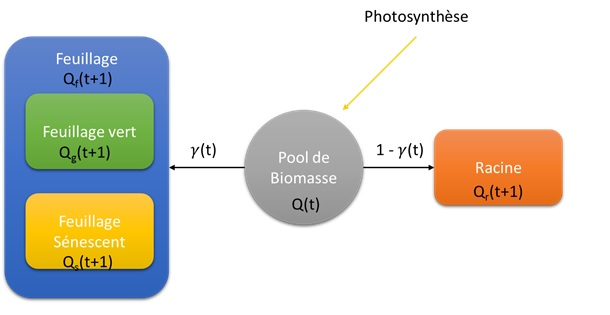
\includegraphics[scale=1.0]{./img/sBeetRoot.jpg}
   \caption{Schéma du modèle LNAS appliqué à la betterave}
   \label{fig:sBeetRoot}
   
   \end{center}
 \end{figure}
 
Production de Biomasse :
 \[ \mathrm{Q}(t) = \big(\mu\cdot\mathrm{PAR}(t)(1-e^{-\lambda\mathrm{Q_g}(t)}\big)\cdot(1+\mathrm{\eta_Q}(t)) \]
 
Allocation au feuillage :
 \[ \mathrm{Q_f}(t+1) = \mathrm{Q_f}(t) + \mathrm{\gamma}(t)\cdot\mathrm{Q}(t) \]
 
Allocation à la racine :
 \[ \mathrm{Q_r}(t+1) = \mathrm{Q_r}(t) + (1 -\mathrm{\gamma}(t))\cdot\mathrm{Q}(t) \]
 
Fonction d'allocation :
 \[ \mathrm{\gamma}(t) = (\gamma_0 + (\gamma_f - \gamma_0)\cdot\mathrm{G_a}(\mathrm{\tau}(t)))\cdot(1+\mathrm{\eta_{\gamma}}(t)) \]
 
Fonction de sénescence :
 \[ \mathrm{Q_s}(t) = \mathrm{G_s}(\mathrm{\tau}(t)- \tau_{sen})\mathrm{Q_f}(t) \]
 
Part de la biomasse produite qui arrive aux feuilles vertes :
 \[\mathrm{Q_g}(t) = \mathrm{Q_f}(t) - \mathrm{Q_s}(t) \]
 
 \begin{itemize}
 
 \item $\mathrm{Q}(t)$ : Production de biomasse au jour t par unité de surface.
 \item $\mu$ : Efficacité énergétique
 \item $1-e^{-\lambda\mathrm{Q_g}(t)}$ : Fraction des radiations interceptées
 \item $\mathrm{PAR}(t)$ : quantité de radiations photosynthétiquement actives par unité de surface.
 \item $\lambda$ : paramètre
 \item $\mathrm{Q_g}(t)$ : masse total des feuilles vertes au jour t
 \item $\mathrm{Q_f}(t)$ : masse total du feuillage au jour t
 \item $\mathrm{Q_s}(t)$ : masse total du feuillage sénescent au jour t 
 \item $\mathrm{\gamma_0}, \mathrm{\gamma_f}$ : paramètres
 \item $\mathrm{\eta}(t)$ : variables aléatoires normales 
 \item $\mathrm{G}(t)$ : variables aléatoires lognormales
 \item $\mathrm{\tau}(t)$ : temps thermique au jour t (température cumulée depuis l'émergence de la plante)
 \item $\tau_{sen}$ : temps thermique où la sénescence commence.
 \item Les paramètres des variables aléatoires font parti des paramètres du modèle.
 
 \end{itemize}
 
\subsection{Modèle LNAS blé}
Nous décrivons ici succinctement le modèle LNAS (Long Normal Allocation and Senescence) appliqué au blé qui est similaire au modèle de la betterave mais plus complexe car plus de compartiments sont modélisés, ainsi que les notions de stres hydrique et thermique et toute la problématique d'humidité du sol. 
C’est aussi un modèle Markovien en temps discret.

Le modèle décrit comment la biomasse produite quotidiennement est allouée aux différents organes avec des fonctions d'allocations propres à chaque types d'organes :
\[ o = \{\mathrm{g:grain, s:tige, r:racines, g : feuilles~vertes}\} \]

La circulation de la biomasse est décrite par trois fonctions $\alpha$,$\beta$ et $\gamma$ qui représentent respectivement l'allocation de la biomasse disponible à chaque type d'organe, la remobilisation de la biomasse d'un organe dans le pool commun de biomasse et la sénescence d'un organe.

\begin{figure}[h]
\centering
  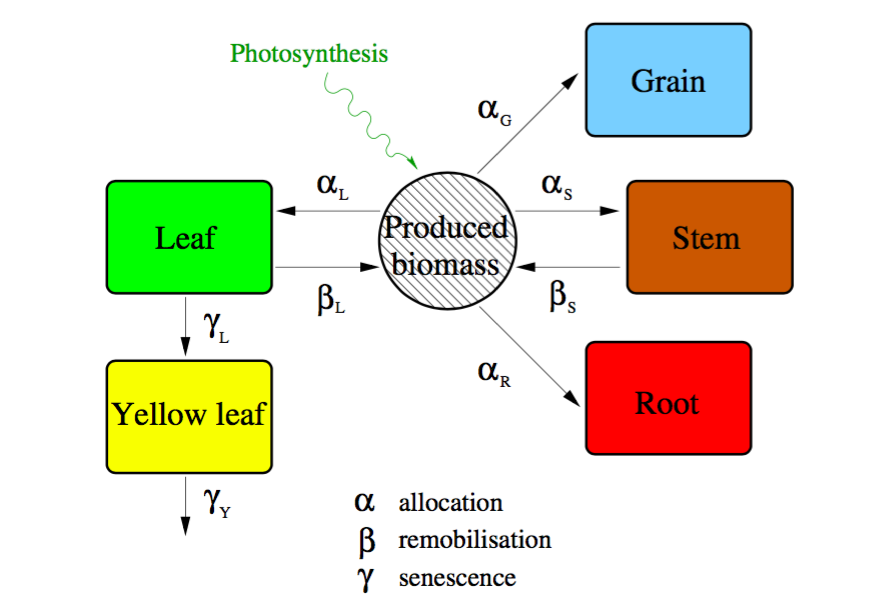
\includegraphics[scale=0.37]{./img/schema-lnas.png}
  \caption{Modélisation de la circulation de biomasse au sein de la plante (modélisée comme un ensemble de compartiments d'organes différents) par des fonctions d'allocation, de remobilisation et de sénescence.}
  \label{fig:circulation_biomasse}
\end{figure}



A chaque temps $n$, on redistribue la biomasse disponible, notée $q^{(n)}$, qui est la somme de la biomasse produite par photosynthèse et de la biomasse réallouée par les organes.

On formalise ce modèle par leurs expressions mathématiques : 
la biomasse de l'organe o, noté $Q_o$ est donnée par :
\[ {Q_o^{(n+1)}} = (1-\beta_o^{(n)}-\gamma_o^{(n)} )(Q_o)^{(n)} +\alpha_o^{(n)}q^{(n)} \]

On accède ainsi à chaque instant à la biomasse des feuilles par exemple grâce à $Q_l$

En supposant que la répartition de biomasse ne commence qu'après un temps caractéristique $\tau_g$ nous pouvons paramétrer la fonction d'allocation $\alpha$ avec la loi log-normale :
\[ {\alpha_g^{(n)}}=F_{\log N(\mu_s,\sigma_g)}(\tau^{(n)}-\tau_g)=\frac{1}{2} (1+\erf[\frac{1}{\sigma_g \sqrt{2}}\log\left(\frac{\tau^{(n)}-\tau_g}{t_{1/2}-\tau_g}\right) \]

Les autres fonctions d'allocations $\beta$ et $\gamma$   peuvent se déduire de l'expression de $\alpha_g^{(n)}$.
Ces trois fonctions $\alpha$, $\beta$ et $\gamma$ sont paramétrées par rapport au temps thermique qui peut s'écrire :

\[ {\tau}^{(n+1)}=\tau^{(n)}+\max[0,\underline{T}^{(n)}-Tc] \]

La quantité de biomasse disponible au jour n est donnée par l'expression de $q^{(n)}$ :
\[ 
{q^{(n)}} = \text{RUE}\cdot \min[SSI^{(n)}, TSI_\uparrow^{(n)}]\underline{PAR}^{(n)}(1-e^{-\lambda LAI^{(n)}})+\sum_o \beta_o^{(n)}Q_o^{(n)} 
\]

Nous nous baserons sur un document fourni par le client lors de l'implémentation de ce modèle, ce document contenant les formules mathématiques nécessaires.

Pour plus de détails et d'explications le lecteur se réfèrera à l'Annexe \ref{ann:LNASble}.
